Codeigniter adalah sebuah framework untuk web yang dibuat dalam format PHP. Format yang dibuat ini selanjutnya dapat digunakan untu membuat sistem aplikasi web yang kompleks. Codeigniter dapat mempercepat proses pembuatan web, karena semua class dan modul yang dibutuhkan sudah ada dan programmer hanya tinggal menggunakannya kembali pada aplikasi web yang akan dibuat \cite{prabowo2015website}.

\section{Tutorial Install CodeIgniter 3}
\begin{enumerate}
	\item Pertama download Framework CodeIgniter di \textbf{\textit{https://www.codeigniter.com/}}
	
	\item Setelah mengunduh file CodeIgniter 3, ekstrak file tersebut menggunakan WinRAR atau 7Zip kedalam folder htdocs jika kamu menggunakan XAMPP atau \textit{/var/www/html}. jika kamu menggunakan Apache2 Standalone, setelah itu ubahlan nama foldernya menjadi namaapplikasi.
	
	\item Sekarang silahkan Kamu coba akses URL \textbf{\textit{http://localhost/ namaaplikasi/}} melalui browser Kamu, akan langsung ditampilkan halaman awal Codeigniter yang berarti Instalasi telah berhasil.
	\begin{figure}[!htbp]
		\centering
		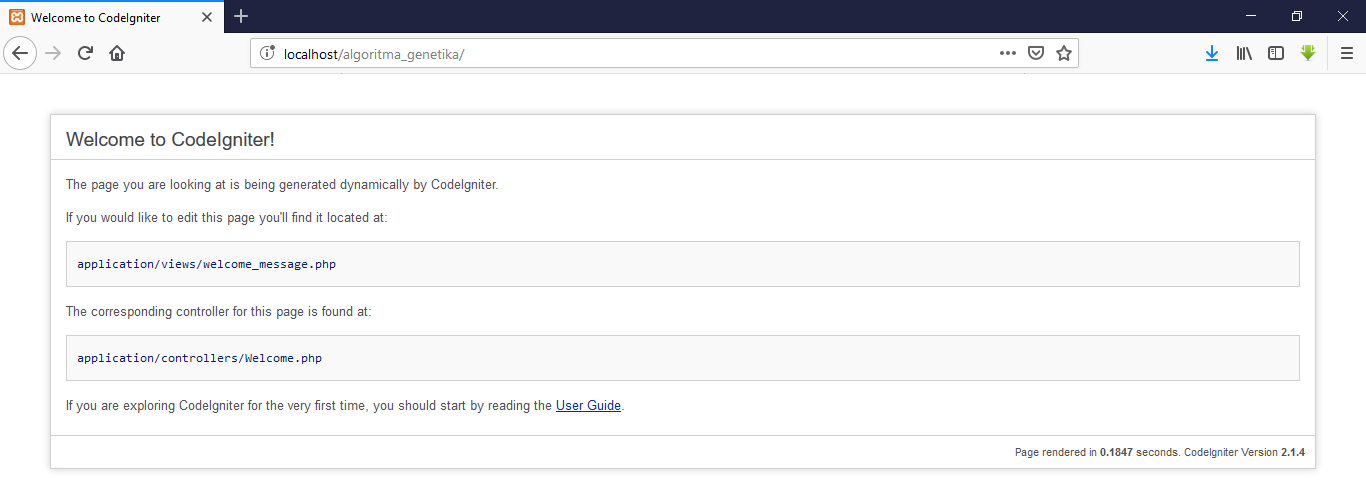
\includegraphics[width=0.5\textwidth]{figures/CodeIgniter1.PNG}
		\label{Xampp2}
	\end{figure}
\end{enumerate}

\section{Struktur CodeIginter}
\begin{enumerate}
	\item Folder Application, merupakan folder yang pada dasarnya menyimpan aplikasi yang sedang kita buat
	\item Folder Cache, merupakan folder yang menyimpan semua cache yang dibuat oleh cache library
	\item Folder Config, merupakan folder yang menyimpan informasi mengenai konfigurasi aplikasi seperti autoload, database, routes dan lainnya.
	\item Folder Controller, merupakan folder menyimpan controller - controller aplikasi yang dapat digunakan untuk menyusun aktivitas program .
	\item Folder Core, adalah folder untuk memperluas class class inti codeigniter.
	\item Folder Helpers, merupakan folder untuk menyimpan helpers.
	\item Folder Hooks, merupakan folder untuk menyimpan hooks untuk mengubah alur fungsi dari core Codeigniter
	\item Folder Language, merupakan folder untuk menyimpan bahasa - bahasa yang akan digunakan.
	\item Folder Libraries, merupakan folder untuk menyimpan library.
	\item Folder Logs, merupakan folder untuk menyimpan semua error log apabila error log diaktifkan.
	\item Folder Models, merupakan folder untuk menyimpan models yang akan mendefinisikan tabel dari database yang dapat kita gunakan oleh Controller yang kita buat untuk mengakses database.
	\item Folder Third-party, merupakan folder untuk menyimpan fungsi fungsi tambahan dalam cara kerja codeigniter.
	\item Folder Views, merupakan folder untuk menyimpan tampilan dari aplikasi yang kita buat.
	\item Folder System, merupakan folder untuk menyimpan sistem inti dari Codeigniter.
\end{enumerate}

\section{Konfigurasi CodeIgniter 3}